\subsection{Cloud Computing Modelle}

\begin{figure}[h]
    \centering
    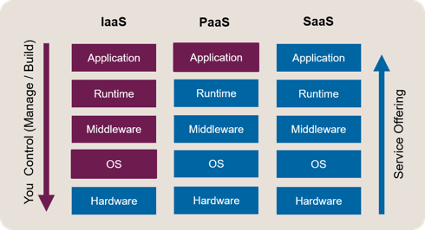
\includegraphics[scale=0.9]{sections/cloud-computing/images/models.png}
    \caption{Modelle}
\end{figure}

\subsubsection{Infrastructure as a Service (IaaS)}

Infrastructure as a Service stellt sowohl virtuelle und physische Server als auch Netzwerk- und Speicherressourcen nach Verlangen des Verbrauchers zur Verfügung. Der Nutzer hat volle Kontrolle über Ressourcen in Bezug auf Speicher und Rechenleistung. Die Auswahl des Betriebssystems wird ebenfalls dem Nutzer überlassen. Beispiel dafür sind Amazon EC2-Cluster und Microsoft Azure. Cloud Storage ist in ähnlicher Weise ein spezieller Fall von IaaS.

\subsubsection{Platform as a Service (PaaS)}

Diese Form des Cloud Computing gibt den Kunden die Möglichkeit, seine Anwendungen auf einer, vom Dienstleistungsgeber, gehosteten Plattform zu entwickeln, bereitzustellen und zu verwalten. Bei diesem Modell handhabt der Dienstleister sämtliche Ressourcen, wie z.B.: Speicher und Rechenleistung. Die Anwendung wird den potenziellen Nutzern über APIs (Application Programming Interface) zur Verfügung gestellt. Hierbei ist wichtig das der Verbraucher keinerlei Kontrolle über die zugrunde liegende Infrastruktur hat. Bekannte Beispiele hierfür sind Web-Hosting Dienste, wie Microsoft Azure Web und Amazon Web Services.

\subsubsection{Software as a Service (SaaS)}

Bei SaaS wird den Nutzern die Möglichkeit gegeben auf eine, vom Dienstleister in der Cloud Infrastruktur bereitgestellten Anwendung zu zugreifen und zu benutzen. Benutzer können dann über eine webbasierte Schnittstelle oder andere, wie ftp und clientseitige Schnittstellen darauf zugreifen. Solche Anwendungen werden gegen monatliche oder jährliche Zahlungen dem Benutzer bereitgestellt. Dabei hat der Verbraucher aber keine bis wenig Kontrolle über im Hintergrund geregelte Ressourcen. Beispiele hierfür sind Microsoft Office 365, Microsoft Skype und Google Apps.